\section{The basic basics}

\begin{frame}

\frametitle{About git\footnote{\emph{git} means "unpleasant person" in British slang. Linus: "I'm an egotistical\\bastard, and I name all my projects after myself."}}
	
\begin{itemize}
	\item A \emph{distributed} version control system (VCS) 
	\item Developed in 2005 by Linus Torvalds (in a single weekend!) to support Linux kernel development
	\item Git was never meant to be used directly :)
	\item Very powerful and very complex
	\item Supports different workflows
	\item We'll be using the GitHub workflow (more or less)	
\end{itemize}
	
\end{frame}

% -----------------------------------------------------------------------------

\begin{frame}

\frametitle{VCS requirements}
	
\begin{block}{Basic requirements}
	\begin{itemize}
		\item Keep track of changes to our code
		\item Facilitate collaboration
	\end{itemize}
\end{block}
	
\begin{block}{Additional requirements}
	\begin{itemize}
		\item Work offline
		\item Support a distributed workflow
		\item Compatibility with existing protocol (e.g. ssh, http)
		\item Cryptographic authentication of history
		\item Efficiency
	\end{itemize}
\end{block}

\end{frame}

% -----------------------------------------------------------------------------

\begin{frame}

\frametitle{Basic terms: repository and commit}
\begin{block}{Repository (repo)}
	A place where your work is kept. It contains your code and its complete history, stored as a collection of commits.
\end{block}

\begin{block}{Commit}
	A basic unit of work in a project. Contains the set of changes, a textual description of what these changes do, a reference to the previous state (the \textit{parent commit}), and the author name and date.\\ \smallskip Finally, the commit contains an alphanumeric identifier (SHA-1 hash), generated from the above information, which is used to uniquely identify the commit. \\For example: \textcolor{Maroon}{\texttt{bdfa760c07d8f621ff603a2dc5d6de810cd62e88}}
\smallskip

You can also use a prefix of the identifier to refer to this commit, usually 5 or 7 characters long, e.g. \textcolor{Maroon}{\texttt{bdfa760}}.
\end{block}
\end{frame}

% -----------------------------------------------------------------------------

\begin{frame}

\frametitle{Getting started on Github}

To begin working on a project using Github, you have to create a repository. There are two ways to do this:


\begin{itemize}
	\item Create an empty repository
	\begin{itemize}
	\item When starting from scratch
	\end{itemize}	
	
	\medskip
	\item Fork another repository
	\begin{itemize}
	\item When you wish to improve and build upon another repository
	\item This creates your personal copy of the repository in which you can make your own commits
	\end{itemize}
\end{itemize}

\end{frame}

% -----------------------------------------------------------------------------

\begin{frame}[fragile]

\frametitle{Making a Github fork and adding a collaborator}


\begin{block}{Task: Fork the example repository}

	To fork a repository, simply click the 
\includegraphics[scale=0.35]{fork} \, icon in the top right corner of the repository webpage. For this tutorial, you will need to clone the \href{https://github.com/larics/git-tutorial-code.git}{larics/git-tutorial-code} repository.
\end{block}

\begin{block}{Task: Add a collaborator to your forked repository}
In the GitHub user interface, on the 
\includegraphics[scale=0.35]{settings} \, tab of your forked repository, select the \texttt{Collaborators and teams} menu and add your partner as a collaborator with \texttt{Write} access.
\end{block}

\end{frame}

% -----------------------------------------------------------------------------

\begin{frame}[fragile]

\frametitle{Cloning and repository structure}

\begin{block}{Cloning}
Cloning creates a local copy of the repository, which includes all the commits in the repository -- the whole history.
\begin{minted}{console}
> git clone git@github.com:<you>/git-tutorial-code.git
\end{minted}
\end{block}

What is contained in the repository directory?
	
\begin{minted}{console}
> cd git-tutorial-code
> ls -la
> git status
\end{minted}
	
\begin{itemize}
	\item The \textit{working tree} -- current version of files ("checked out")
	\item The hidden \texttt{.git} folder which contains repository metadata \\ (all the commits, and the internal structures for storing them)
	\item The \texttt{git status} command provides an overview of what is going on in your repository.
\end{itemize}
\begin{minted}{console}
\end{minted}
	
\end{frame}

% -----------------------------------------------------------------------------

\begin{frame}[fragile]
	\frametitle{Your first commit}
	
	\begin{block}{Task}
	Open \texttt{README.md} and add the following lines, then save the file:
	\begin{minted}{text}
Maintainers:
  <your name>
	\end{minted}
	\end{block}

Run the following, and observe what is happening.

	\begin{minted}{console}
> git status
> git diff
> git add README.md
> git status
> git gui
> git commit -m "Add maintainer."
> git status
> git log
	\end{minted}
	
\end{frame}

% -----------------------------------------------------------------------------

\begin{frame}[fragile]

\frametitle{Making a commit - recap}
	
\begin{enumerate}
	\item Make a change in the working tree. For example:
	\begin{itemize}
	\item Edit a file
	\item Create a file
	\item Delete a file 
	\item Move a file (git considers moving as deleting + creating a new file)
	\end{itemize}
	\item \texttt {git add} the change to the \textit{staging area} ("index")
	\item Perform a final inspection of the staged changes
	\begin{itemize}
	\item \texttt{git gui} is handy for this
	\item The staged changes should make a logically grouped set of changes
	\item Feel free to make as many commits as you like
	\item "Commit early and often"
	\end{itemize}
	\item \texttt{git commit} your changes
	\begin{itemize}
	\item  "50/72" rule - the title of the commit description should be {\raise.17ex\hbox{$\scriptstyle\sim$}}50 characters, the body should be wrapped to 72 characters
	\item Use the imperative form as the first word in the title -- e.g. \\"Add prime checking", "Implement saving to file", "Fix broken build"
	\end{itemize}
\end{enumerate}
	
\end{frame}

% -----------------------------------------------------------------------------

\begin{frame}[fragile]

\frametitle{Making a commit - 2}

\begin{block}{Managing staged changes}
	To unstage all changes, use \texttt{git reset}. You can finely tune what goes into the commit by staging/unstaging individual lines using \texttt{git gui}. (For those who prefer the command line, you can use the \texttt{-p} switch of \texttt{git add} and \texttt{git reset}).
\end{block}

\begin{block}{Task: Adding a license and \texttt{.gitignore}}
	Add a license to the project. Create a \texttt{LICENSE.txt} file and copy the \href{https://choosealicense.com/licenses/apache-2.0/}{Apache License 2.0 text} into this file. Create a \texttt{.gitignore} file, with the following two lines:
	\begin{minted}{text}
cpp/build/
*.pyc
	\end{minted}
Make two separate commits, one for adding the license, and the other for adding \texttt{.gitignore}.
\end{block}
	
\end{frame}

% -----------------------------------------------------------------------------

\begin{frame}[fragile]
	\frametitle{Discarding unstaged changes}
	
	\begin{block}{Task}
	Delete a big chunk of text from \texttt{README.md}. Do not add or commit.
	\end{block}
	
	To find out what is going on, use \texttt{git status}.
	\bigskip
	
    Revert the changes by retrieving ("checking out") the last commited version of the file (can also be a directory) using the \texttt{checkout} command:

	\begin{minted}{console}
> git checkout README.md
	\end{minted}
	
	Note that the checked out version will contain the staged changes.
\end{frame}
% -----------------------------------------------------------------------------
\begin{frame}[fragile]

\frametitle{Discarding many unwanted changes}

If you have made many changes in your working tree, spanning several files, you can discard all of them at once (this also includes the staged changes) with the \texttt{git reset --hard} command.

\medskip
This will restore all tracked files in the working tree to the most recently committed version (this commit is also known as the \texttt{HEAD} commit).

\begin{block}{Task: Discarding several unwanted changes}
Delete several files from the cloned example repository. Check the output of \texttt{git status}. Do not add or commit the changes. To discard all changes at once, run:
\begin{minted}{console}
> git reset --hard
\end{minted}

\end{block}

\end{frame}

% -----------------------------------------------------------------------------


\begin{frame}[fragile]

\frametitle{Going back in time}

The point of using a version control system such as git is the ability to retrieve older versions of files in the project.

	\begin{block}{Task}
	Delete a big chunk of text from \texttt{cpp/CMakeLists.txt}. Commit.
	\end{block}
	
	Git allows you to retrieve another version of a file from an earlier commit.\footnote{writing good commit messages is important, because it will make identifying \\the right commit much easier} To identify the desired commit, use the \texttt{gitg} tool, or run \texttt{git log} (add \texttt{--oneline} for an abbreviated list of commits). Then, run:
	\begin{minted}{console}
> git checkout <commit ID> <file>
	\end{minted}
	Git will place the checked out version of the file in the working tree, and will also stage the changes for you.
\end{frame}

% -----------------------------------------------------------------------------

\begin{frame}[fragile]

\frametitle{Reverting previous commits}

Another benefit of splitting the work in different commits is the ability to undo them using \texttt{git revert}.

	\begin{block}{Task}
	Discard the earlier version of the file \texttt{cpp/CMakeLists.txt} that you have just checked out:
	\begin{minted}{console}
> git reset --hard
	\end{minted}

	Revert the offending commit:
	\begin{minted}{console}
> git revert <commit ID>
	\end{minted}

Reverting generates an \textit{inverse commit}, which has the exactly opposite set of changes.
	\end{block}

\end{frame}

% -----------------------------------------------------------------------------

\begin{frame}[fragile]

\frametitle{Amending the last commit}

In the special case when you want to add aditional changes to the \textit{last commit} that you have made, \textbf{and if you have not yet pushed that commit}:

	\begin{enumerate}
	\item Stage the additional changes using \texttt{git add}
	\item Inspect the changes, as previously described
	\item Run \texttt{git commit --amend}
	\end{enumerate}

In case you only wish to amend the commit description, just run \texttt{git commit --amend}, without staging any changes.

	\begin{block}{Task}
	Amend the description of the revert commit that you have just made:
	\begin{minted}{text}
Undo the destructive changes that the cat has commited by
walking on the keyboard.
	\end{minted}
\end{block}

\end{frame}

% -----------------------------------------------------------------------------



\begin{frame}[fragile]
	\frametitle{Visualizing git operation}
	
	\begin{figure}
		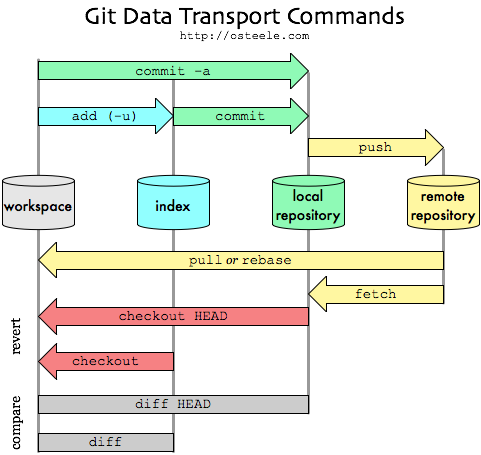
\includegraphics[scale=0.4]{git-transport}
	\end{figure}
\end{frame}

% -----------------------------------------------------------------------------

\begin{frame}[fragile]
	\frametitle{Pushing the changes to the remote repository}
	
	\begin{block}{Local vs. remote changes}
	\texttt{commit} only saves changes \alert{locally}! The command \texttt{git push} is used to upload the commits you have made to a remote repository. 
	
	\begin{minted}{console}
> git push origin master
	\end{minted}
	\end{block}

Note that you can simply call \texttt{git push} if you have set up your local branch to be a tracking branch (which will be explained later; in most cases, git will already have automatically configured this for you).

	\begin{block}{Collaboration issues}
What happens when somebody else pushed changes to the remote repository before us? In this case, git refuses to push. We must synchronize our local repository first!
	\end{block}	
	
\end{frame}

% -----------------------------------------------------------------------------


\begin{frame}[fragile]
	\frametitle{Dealing with conflicts: fetching changes}

	\begin{block}{Task}
	Both teammates have changed the same file. The person whose push failed has to resolve the conflict.	
	\end{block}
	
	Getting changes is a two-step process:
	\begin{enumerate}
		\item \texttt{fetch} the changes from the remote repository
		\item \texttt{merge} the changes into your working tree
	\end{enumerate}
	
	\begin{minted}{console}
> git fetch
> git status
> git diff master origin/master
	\end{minted}
	
	\begin{block}{Understanding \texttt{diff}}
	\texttt{git diff a b} shows changes that need to be applied to \texttt{a} to make it the same as \texttt{b}. \texttt{a} and \texttt{b} are references to any two commits.
	\end{block}
	
\end{frame}

% -----------------------------------------------------------------------------

\begin{frame}[fragile]
	\frametitle{Dealing with conflicts: merging}
	
	When you call \texttt{merge}, git adds a special merge commit to your local repository, which has two parent commits: your local previous head commit, and the other side's commit (in this case, the \textit{other side} is the same branch in the remote repository).
	\begin{minted}{console}
> git merge origin/master
	\end{minted}
	
	\begin{block}{\texttt{fetch}+\texttt{merge}=\texttt{pull}?}
	\texttt{pull} will do \texttt{fetch} and \texttt{merge} in a single step. However, if \texttt{origin} has changed, you might get yourself into trouble.\footnote{A really nice article advocating the use of \texttt{fetch}+\texttt{merge} can be found on \href{http://longair.net/blog/2009/04/16/git-fetch-and-merge/}{Mark's Blog}} 
	\end{block}
	
\end{frame}

% -----------------------------------------------------------------------------
\begin{frame}[fragile]
	\frametitle{Resolving conflicts}
	
	After merging, the file ends up in a conflicted state:
	\begin{minted}{console}
> git merge origin/master
> git status
> git gui
	\end{minted}	
	
	Conflict markers inside the file:
	\begin{minted}{diff}
<<<<<<< HEAD
Code on working branch before the merge
=======
Code introduced by the merge
>>>>>>> origin/master
	\end{minted}

	To resolve the conflict, manually edit the file, mark resolution by \texttt{git add}, commit and push:
	\begin{minted}{console}
> git add <file name>
> git commit
> git push origin master
	\end{minted}
	
\end{frame}

% -----------------------------------------------------------------------------

\begin{frame}[fragile]
	\frametitle{Handling binary files}
	
	\begin{block}{Difference between text and binary files}
	Changes to text files are stored incrementally, as diffs, which is very space-efficient. For every change in a binary file, the whole file is stored again. The change persists, even after the file is removed!
	\end{block}
	
	\begin{block}{How to handle binary files}
	Storing binary files (e.g. graphics) is ok if they are small and change infrequently. Otherwise, create a README file with instructions for downloading the files (or a download script, if you want to be fancy).
	\end{block}
	
	\begin{block}{Build output}
	\alert{Never} commit build output (even if it is text, e.g. documentation)! It can waste \alert{huge} amounts of space and it will create unnecessary conflicts.
	\end{block}
\end{frame}

% -----------------------------------------------------------------------------

\begin{frame}

\frametitle{Visualizing your repo}

\begin{itemize}
	\item The \texttt{gitg} tool can visualize your repository
	\item GitHub provides similar functionality with the Graphs $\rightarrow$ Network menu.
\end{itemize}

\begin{block}{Task}
	Visualize your repo with \texttt{gitg} and on GitHub. Notice how the repo history is not linear. 
\end{block}

\end{frame}
% -----------------------------------------------------------------------------
